% PART 2 (SECTION 8.2)
\part{Section 8.2}
%%%%%%%%%%%%%%%%%%%%%%%%%%%%%%%%%%%%%%%
\begin{transitionframe}
    \begin{center}
    { 
        \Huge \textcolor{white}{\textbf{Polygons}}
        \\[-1em]
        \noindent\textcolor{white}{\rule{12cm}{0.4pt}}
        
        %\large \textcolor{white}{Section 8.2}
    }
    \end{center}
\end{transitionframe}
%%%%%%%%%%%%%%%%%%%%%%%%%%%%%%%%%%%%%%%
%        SLIDE 
%%%%%%%%%%%%%%%%%%%%%%%%%%%%%%%%%%%%%%%
\begin{frame}{Outline}
    \begin{columns}[t]
        \begin{column}{.5\textwidth}
            \tableofcontents[part=2, sections={1-3}]
        \end{column}
        \begin{column}{.5\textwidth}
            \tableofcontents[part=2, sections={4-5}]
        \end{column}
    \end{columns}
\end{frame}
%%%%%%%%%%%%%%%%%%%%%%%%%%%%%%%%%%%%%%%
%        SLIDE 
%%%%%%%%%%%%%%%%%%%%%%%%%%%%%%%%%%%%%%%
\section{Polygons}
\subsection{What is a Polygon?}
\begin{frame}[t]{What is a Polygon?}
    \begin{itemize}
        \item Polygon is another word derived from Greek meaning ``many angles''.
    \end{itemize}
    %
    \begin{block}{Definition}
        A shape that meets the following conditions are called polygon:
        \begin{itemize}
            \item closed shape
            \item made of only straight lines
            \item 2-Dimensional shape
        \end{itemize}
    \end{block}
    %
    \begin{figure}[H]
        \centering
        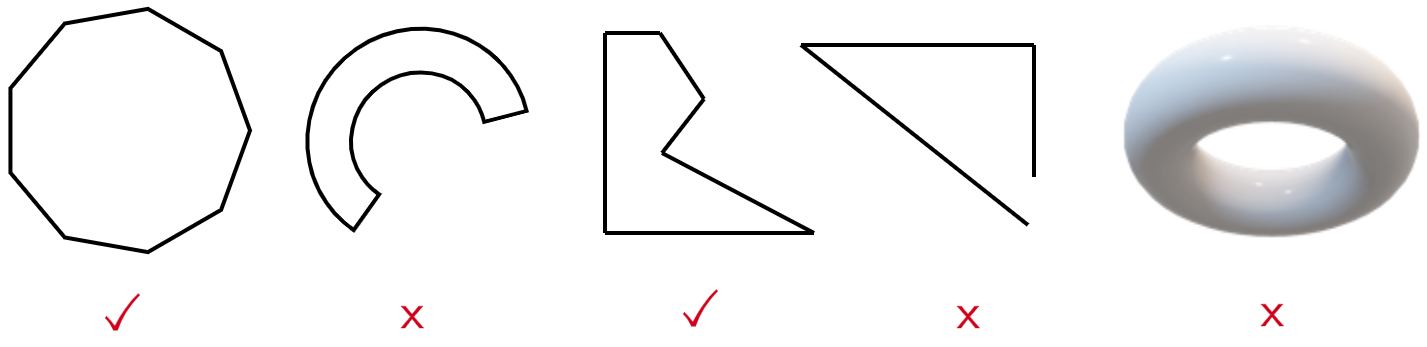
\includegraphics[scale=0.2]{pics/polygons.png}
    \end{figure}
\end{frame}
%%%%%%%%%%%%%%%%%%%%%%%%%%%%%%%%%%%%%%%
%        SLIDE 
%%%%%%%%%%%%%%%%%%%%%%%%%%%%%%%%%%%%%%%
\subsection{Sides and Vertices}
\begin{frame}{Sides and Vertices}
    \begin{itemize}
        \item Each straight-line segments are called \textit{sides}.
        \item A point where two sides meet is called a \textit{vertex (plural Vertices)}.
    \end{itemize}
    %
    \begin{figure}[H]
        \centering
        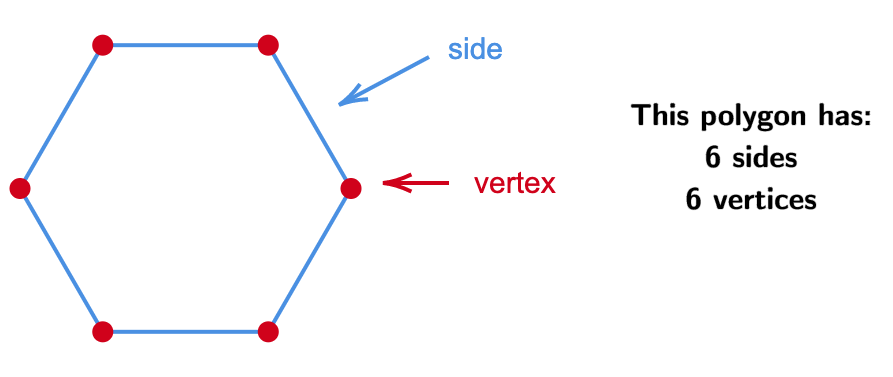
\includegraphics[scale=0.35]{pics/sides_vertices.png}
    \end{figure}
\end{frame}
%%%%%%%%%%%%%%%%%%%%%%%%%%%%%%%%%%%%%%%
%        SLIDE 
%%%%%%%%%%%%%%%%%%%%%%%%%%%%%%%%%%%%%%%
\subsection{Interior and Exterior Angles}
\begin{frame}[t]{Interior and Exterior Angles}
    \begin{columns}[t]
    %
    \column{0.45\textwidth}
    \textbf{Interior Angles}
    \begin{itemize}
        \item An angle formed by two adjacent sides inside the polygon.
    \end{itemize}
    %
    \column{0.45\textwidth}
    \textbf{Exterior Angles}
    \begin{itemize}
        \item An angle at a vertex of the polygon, outside the polygon, formed by one side and the extension of an adjacent side.
    \end{itemize}
    \end{columns}
    %
    \begin{figure}[H]
        \centering
        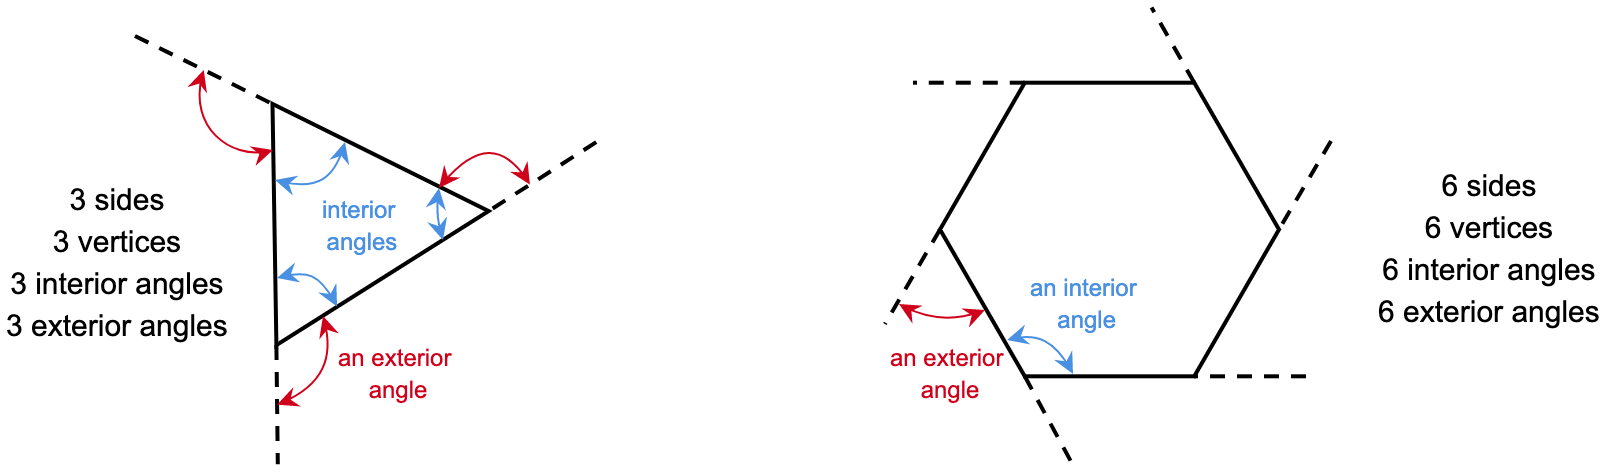
\includegraphics[scale=0.26]{pics/interior_exterior_polygons.png}
    \end{figure}
\end{frame}
%%%%%%%%%%%%%%%%%%%%%%%%%%%%%%%%%%%%%%%
%        SLIDE 
%%%%%%%%%%%%%%%%%%%%%%%%%%%%%%%%%%%%%%%
\subsection{Name of Some Polygons}
\begin{frame}{Name of Some Polygons}
    \begin{itemize}
        \item Polygons are named according to their number of sides.
    \end{itemize}
    %
    \begin{table}[H]
    \centering
    \begin{tabular}{c c || c  c}
        \toprule
        Number of sides & Name &  Number of sides  & Name\\
        \hline
        3 & Triangle        &   8       & Octagon
        \\ 
        4 & Quadrilateral   &   9       & Nanogon
        \\ 
        5 & Pentagon        &   10      & Decagon
        \\  
        6 & Hexagon         &   12      & Dodecagon
        \\
        7 & Heptagon        &   20      & Icosagan
        \\ \bottomrule
    \end{tabular}
    \label{tab:polygons_names}
\end{table}
\end{frame}
%%%%%%%%%%%%%%%%%%%%%%%%%%%%%%%%%%%%%%%
%        SLIDE 
%%%%%%%%%%%%%%%%%%%%%%%%%%%%%%%%%%%%%%%
\subsection{Regular Polygons}
\begin{frame}[t]{Regular Polygons}
    \begin{itemize}
        \item All sides are equal.
        \item All interior angles are equal.
        \item All exterior angles are equal.
    \end{itemize}
    %
    \begin{figure}[H]
        \centering
        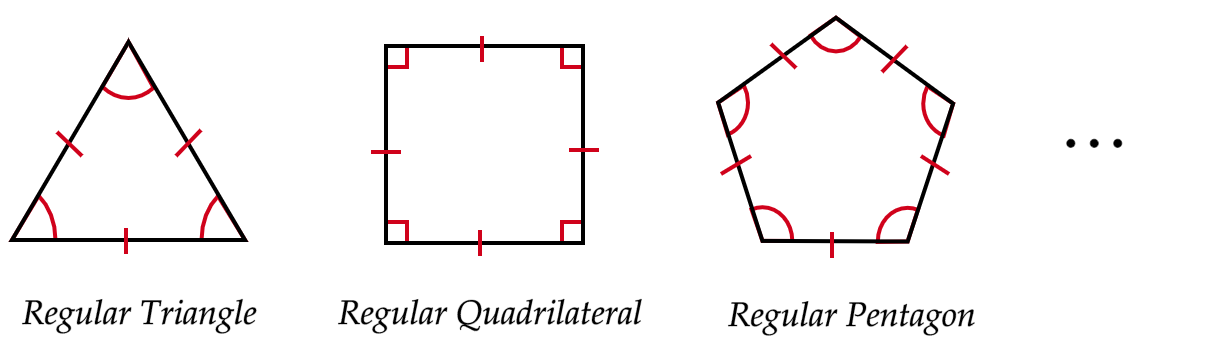
\includegraphics[scale=0.3]{pics/regular_polygon.png}
    \end{figure}
\end{frame}
%%%%%%%%%%%%%%%%%%%%%%%%%%%%%%%%%%%%%%%
%        SLIDE 
%%%%%%%%%%%%%%%%%%%%%%%%%%%%%%%%%%%%%%%
\section{More on Interior Angles}
\subsection{Sum of Interior Angles}
\begin{frame}[t]{Sum of Interior Angles}
    \begin{itemize}
        \item It can be proven that sum of interior angles in a triangle is equal to $180^\circ$.
        \item Using this fact, we can find sum of interior angles in other polygons.
    \end{itemize}
    %
    \begin{figure}[H]
        \centering
        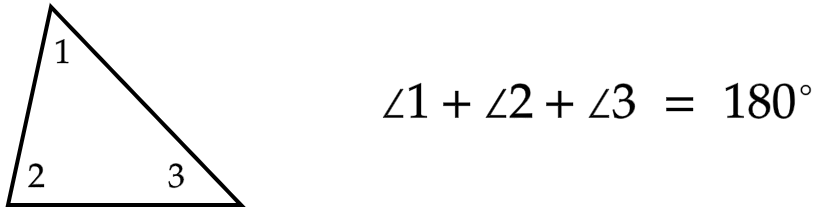
\includegraphics[scale=0.3]{pics/sum_angles_triangle.png}
    \end{figure}
    %
    \begin{itemize}
        \item To find the sum of interior angles in other polygons, we must ask ourselves how many triangles we can create inside a polygons?
        \item Is there any relationship between number of triangles created insides a polygon and number of sides?
    \end{itemize}
\end{frame}
%%%%%%%%%%%%%%%%%%%%%%%%%%%%%%%%%%%%%%%
%        SLIDE 
%%%%%%%%%%%%%%%%%%%%%%%%%%%%%%%%%%%%%%%
\begin{frame}{}
    \begin{figure}[H]
        \centering
        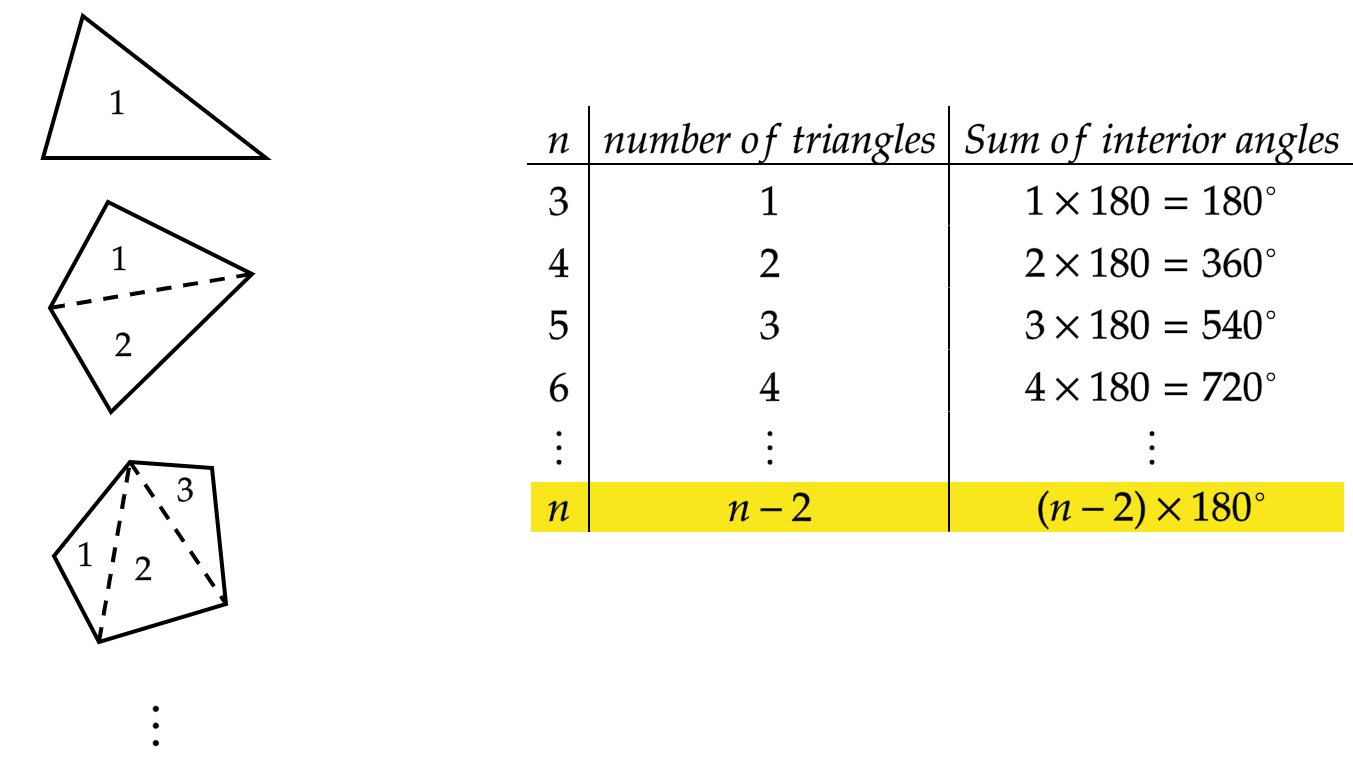
\includegraphics[scale=0.3]{pics/general_sum_of_interior.png}
    \end{figure}
\end{frame}
%%%%%%%%%%%%%%%%%%%%%%%%%%%%%%%%%%%%%%%
%        SLIDE 
%%%%%%%%%%%%%%%%%%%%%%%%%%%%%%%%%%%%%%%
\begin{frame}[t]{Example (Sum of Interior Angles)}
    \begin{example}
        \begin{itemize}
            \item Find sum of interior angles in
            \begin{enumerate}[(a)]
                \item Decagon
                \item Octagon
                \item 30-gon
            \end{enumerate}
        \end{itemize}
    \end{example}
\end{frame}
%%%%%%%%%%%%%%%%%%%%%%%%%%%%%%%%%%%%%%%
%        SLIDE 
%%%%%%%%%%%%%%%%%%%%%%%%%%%%%%%%%%%%%%%
\subsection{An Interior Angle of a Regular Polygon}
\begin{frame}[t]{An Interior Angle of a Regular Polygon}
    \begin{columns}
    \column{0.5\textwidth}
    \begin{itemize}
        \item Consider a regular polygon.
        \item In a regular polygon, all interior angles are equal. 
        \item Thus, we can easily find the measure of an interior angle by dividing the sum of interior angles by number of sides.
    \end{itemize}
    %
    \column{0.45\textwidth}
    \begin{figure}[H]
        \centering
        
\includegraphics[scale=0.05]{pics/bam.jpg}
    \end{figure}
    \end{columns}
    %
    \begin{block}{Measure of an interior angle in a regular polygon}
    An interior angle of a \textbf{regular polygon} can be find as follow:
    \[
        \text{an interior angle of a regular polygon} = \frac{\text{Sum of interior angles}}{\text{Number of sides}}   
        \label{for::interior_angle}    
    \]
    \end{block}
    %
\end{frame}
%%%%%%%%%%%%%%%%%%%%%%%%%%%%%%%%%%%%%%%%%%%%%%%%
%        SLIDE 
%%%%%%%%%%%%%%%%%%%%%%%%%%%%%%%%%%%%%%%%%%%%%%%%
\begin{frame}[t]{Example (Measure of an Interior Angle)}
    \begin{example}
        Find the measure of an interior angle in a regular octagon.
    \end{example}
\end{frame}
%%%%%%%%%%%%%%%%%%%%%%%%%%%%%%%%%%%%%%%%%%%%%%%%
%        SLIDE 
%%%%%%%%%%%%%%%%%%%%%%%%%%%%%%%%%%%%%%%%%%%%%%%%
\section{More on Exterior Angles}
\subsection{Sum of Exterior Angles}
\begin{frame}[t]{Sum of Exterior Angles}
    \begin{itemize}
        \item It can be proven that sum of exterior angles in any polygon (regular or irregular) is always equal to $360^\circ$.
    \end{itemize}
    %
\begin{figure}[H]
    \centering
    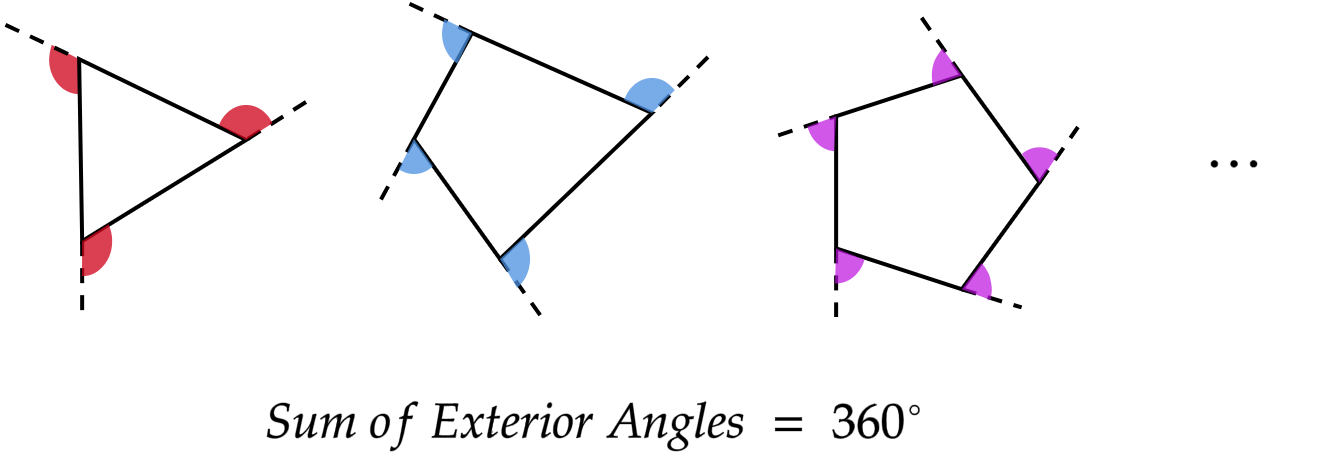
\includegraphics[scale=0.3]{pics/sum_exterior_angles.png}
\end{figure}
\end{frame}
%%%%%%%%%%%%%%%%%%%%%%%%%%%%%%%%%%%%%%%%%%%%%%%%
%        SLIDE 
%%%%%%%%%%%%%%%%%%%%%%%%%%%%%%%%%%%%%%%%%%%%%%%%
\subsection{An Exterior Angle of a Regular Polygon}
\begin{frame}[t]{An Exterior Angle of a Regular Polygon}
    %
    \begin{itemize}
        \item In a regular polygon, all exterior angles are equal.
        \item We could measure an exterior angle of a regular polygon by dividing the sum of exterior angles (which is $360^\circ$) by number of sides.
    \end{itemize}
    %
    \begin{block}{Measure of an exterior angle in a regular polygon}
    An exterior angle of a \textbf{regular polygon} can be find as follow:
    \[
        \text{an exterior angle of a regular polygon} = \frac{360^\circ}{\text{Number of sides}}   
        \label{for::exterior_angle}    
    \]
    \end{block}    
\end{frame}
%%%%%%%%%%%%%%%%%%%%%%%%%%%%%%%%%%%%%%%%%%%%%%%%
%        SLIDE 
%%%%%%%%%%%%%%%%%%%%%%%%%%%%%%%%%%%%%%%%%%%%%%%%
\begin{frame}[t]{Example (Measure of an Exterior Angle)}
    \begin{example}
        \begin{itemize}
            \item Find an exterior angle of the following regular polygons:
            \begin{enumerate}
                \item A regular hexagon
                \item A regular octagon
                \item A 14-gon
            \end{enumerate}
        \end{itemize}
    %
    \end{example}
\end{frame}
%%%%%%%%%%%%%%%%%%%%%%%%%%%%%%%%%%%%%%%
%%%%%%%%%%%%%%%%%%%%%%%%%%%%%%%%%%%%%%%%%%%%%%%%
%        SLIDE 
%%%%%%%%%%%%%%%%%%%%%%%%%%%%%%%%%%%%%%%%%%%%%%%%
\section{Triangles}
\begin{frame}{Triangles}
    \begin{itemize}
        \item There are 6 types of triangles. 
    \end{itemize}
    %
    \begin{figure}[H]
        \centering
        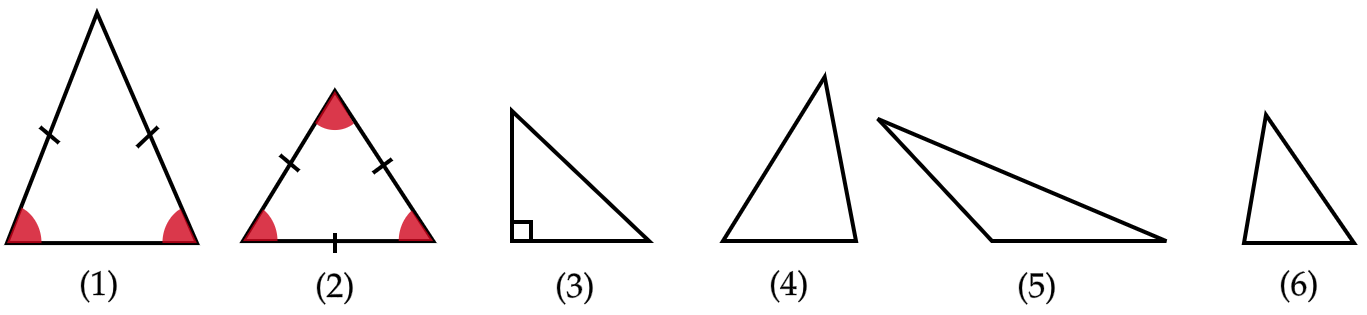
\includegraphics[scale=0.3]{pics/types_of_triangles.png}
    \end{figure}
\end{frame}
%%%%%%%%%%%%%%%%%%%%%%%%%%%%%%%%%%%%%%%%%%%%%%%%
%        SLIDE 
%%%%%%%%%%%%%%%%%%%%%%%%%%%%%%%%%%%%%%%%%%%%%%%%
\subsection{Isosceles Triangle}
\begin{frame}{Isosceles Triangle}
    \begin{itemize}
        \item Isosceles means ``same legs'' in Greek.
        \item Two sides are equal.
        \item The angles opposite the equal sides are also equal.
    \end{itemize}
    %
    \begin{columns}
    \column{0.45\textwidth}
        \begin{figure}[H]
        \centering
            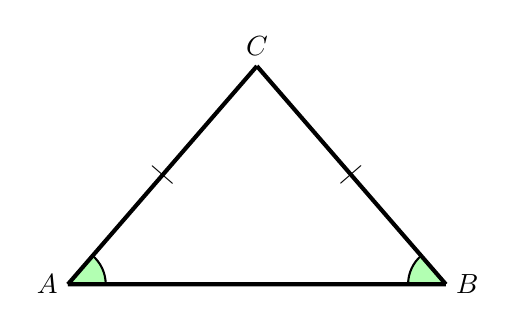
\begin{tikzpicture}[scale=0.8]
            \coordinate[label=left:$A$]  (A) at (-1,0);
            \coordinate[label=right:$B$] (B) at (5,0);
            \coordinate[label=above:$C$] (C) at (2,3.464);
    
            % angle CAB
            \begin{scope}[shift={(-1cm,0cm)}]
                \draw[fill=green!30] (0,0) -- (0:0.6cm) arc (0:50:0.6cm);
            \end{scope}
            % angle CBA
            \begin{scope}[shift={(5cm,0cm)}]
                \draw[fill=green!30] (0,0) -- (-180:0.6cm) arc (180:130:0.6cm);
            \end{scope}
            % triangle
            \draw [line width=1.5pt] (A) --  (B)
                                     (A) -- node[sloped] {$|$} (C)
                                     (B) -- node[sloped] {$|$} (C);
          \end{tikzpicture}
        \label{fig:isosceles_triangle}
    \end{figure}
    %
    \column{0.45\textwidth}
        \begin{align*}
            \overline{AC} &= \overline{BC}
            \\
            \angle A &= \angle B
        \end{align*}
    \end{columns}
\end{frame}
%%%%%%%%%%%%%%%%%%%%%%%%%%%%%%%%%%%%%%%%%%%%%%%%
%        SLIDE 
%%%%%%%%%%%%%%%%%%%%%%%%%%%%%%%%%%%%%%%%%%%%%%%%
\subsection{Equilateral Triangle}
\begin{frame}{Equilateral Triangle}
    \begin{itemize}
        \item In equilateral triangle, all sides are equal to each other. 
        \item Also all angles are equal and $60^\circ$ each (why?).
    \end{itemize}
    %
    \begin{columns}
    \column{0.45\textwidth}
        \begin{figure}[H]
            \centering
                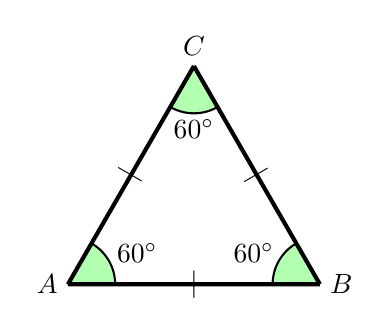
\begin{tikzpicture}[scale=0.8]
                \coordinate[label=left:$A$]  (A) at (0,0);
                \coordinate[label=right:$B$] (B) at (4,0);
                \coordinate[label=above:$C$] (C) at (2,3.464);
                % angle alpha
                \draw[fill=green!30] (0,0) -- (0:0.75cm) arc (0:60:.75cm);
                \draw (1.10cm,0.5cm) node {$60^\circ$};
            
                % angle beta
                \begin{scope}[shift={(4cm,0cm)}]
                    \draw[fill=green!30] (0,0) -- (-180:0.75cm) arc (180:120:0.75cm);
                    \draw (-1.05cm, 0.5cm) node {$60^\circ$};
                \end{scope}
            
                % angle gamma
                \begin{scope}[shift={(60:4)}]
                    \draw[fill=green!30] (0,0) -- (-120:.75cm) arc (-120:-60:.75cm);
                    \draw (-90:1cm) node {$60^\circ$};
                \end{scope}
            
                % the triangle
                \draw [line width=1.5pt] (A) --  node[sloped] {$|$} (B)
                                         (A) --  node[sloped] {$|$} (C)
                                         (B) --  node[sloped] {$|$} (C);
              \end{tikzpicture}
            \label{fig:equilateral_triangle}
    \end{figure}
    %
    \column{0.45\textwidth}
        \begin{align*}
            \overline{AC} &= \overline{BC} = \overline{AB}
            \\
            \angle A &= \angle B = \angle C = 60^\circ
        \end{align*}
    \end{columns}
\end{frame}
%%%%%%%%%%%%%%%%%%%%%%%%%%%%%%%%%%%%%%%%%%%%%%%%
%        SLIDE 
%%%%%%%%%%%%%%%%%%%%%%%%%%%%%%%%%%%%%%%%%%%%%%%%
\subsection{Right Triangle}
\begin{frame}{Right Triangle}
    \begin{itemize}
        \item One angle is right angle ($90^\circ$).
        \item Hypotenuse is the largest side ($c$). It is always opposite of right angle.
        \item The other side is called legs.
        \item \alert{It is very important to identify which one is hypotenuse!!}
    \end{itemize}
    %
    \begin{columns}
    \column{0.45\textwidth}
        \begin{figure}[H]
            \centering
                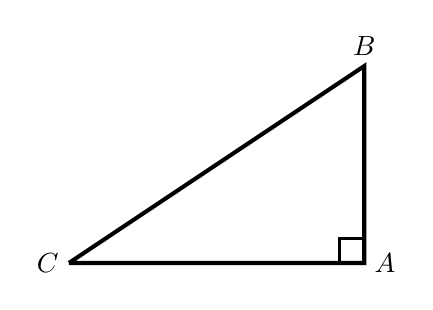
\begin{tikzpicture}[scale=1.25]
                    \coordinate [label=left:$C$]  (C) at (-1.5cm,-1.0cm);
                    \coordinate [label=right:$A$] (A) at (1.5cm,-1.0cm);
                    \coordinate [label=above:$B$] (B) at (1.5cm,1.0cm);
                    \draw [line width=1.5pt] (C) -- (B) -- (A) -- (C);
                    \draw [line width=1pt] (1.25cm,-1.0cm) rectangle (1.5cm,-0.75cm);
                \end{tikzpicture}
            \label{fig:right_triangle}
        \end{figure}
    %
    \column{0.45\textwidth}
        \begin{align*}
            & \text{$\overline{BC}$ is hypotenuse}
            \\
            & \angle A = 90^\circ
        \end{align*}
    \end{columns}    
\end{frame}
%%%%%%%%%%%%%%%%%%%%%%%%%%%%%%%%%%%%%%%%%%%%%%%%
%        SLIDE 
%%%%%%%%%%%%%%%%%%%%%%%%%%%%%%%%%%%%%%%%%%%%%%%%
\subsection{Scalene, Obtuse, and Acute Triangles}
\begin{frame}[t]{Scalene, Obtuse, and Acute Triangles}
    \begin{columns}[t]
    \column{0.25\textwidth}
        \textbf{Scalene:} 
        
        In this triangle, no two sides nor two angles are equal. 
        \begin{figure}[H]
            \centering
                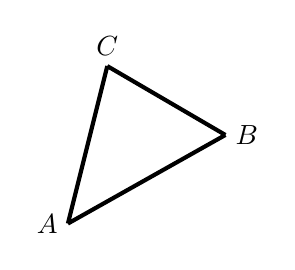
\begin{tikzpicture}[scale=0.5]
                \coordinate[label=left:$A$]  (A) at (0,-1);
                \coordinate[label=right:$B$] (B) at (4,1.25);
                \coordinate[label=above:$C$] (C) at (1,3);
            
                % the triangle
                \draw [line width=1.5pt] (A) --   (B)
                                         (A) --   (C)
                                         (B) --   (C);
              \end{tikzpicture}
            \label{fig:scalene_triangle}
        \end{figure}
    \column{0.33\textwidth}
        \textbf{Obtuse Triangle:} 
        
        One of the angle in this triangle is an obtuse angle; In other words, one angles is between $90^\circ$ and $180^\circ$.
        \begin{figure}[H]
            \centering
                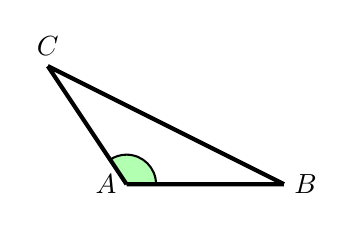
\begin{tikzpicture}[scale=0.5]
                \coordinate[label=left:$A$]  (A) at (0,0);
                \coordinate[label=right:$B$] (B) at (4,0);
                \coordinate[label=above:$C$] (C) at (-2,3);
                % angle alpha
                \draw[fill=green!30] (0,0) -- (0:0.75cm) arc (0:125:.75cm);
                %\draw (0.5cm,1cm) node {$x$};
                
                % the triangle
                \draw [line width=1.5pt] (A) --   (B)
                                         (A) --   (C)
                                         (B) --   (C);
              \end{tikzpicture}
            \label{fig:obtuse_triangle}
        \end{figure}  
    \column{0.33\textwidth}
        \textbf{Acute Triangle}
        
        If all angles are acute angles (less than $90^\circ$), then we have an acute triangle.
        An acute triangle can be equilateral, isosceles or scalene.
        
        \begin{figure}[H]
            \centering
                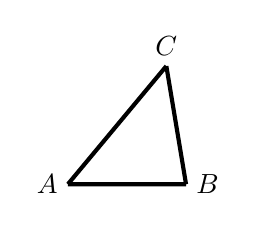
\begin{tikzpicture}[scale=0.5]
                \coordinate[label=left:$A$]  (A) at (0,0);
                \coordinate[label=right:$B$] (B) at (3,0);
                \coordinate[label=above:$C$] (C) at (2.5,3);
            
                % the triangle
                \draw [line width=1.5pt] (A) --   (B)
                                         (A) --   (C)
                                         (B) --   (C);
              \end{tikzpicture}
            \label{fig:acute_triangle}
        \end{figure}
        %
    \end{columns}
\end{frame}
%%%%%%%%%%%%%%%%%%%%%%%%%%%%%%%%%%%%%%%%%%%%%%%%
%        SLIDE 
%%%%%%%%%%%%%%%%%%%%%%%%%%%%%%%%%%%%%%%%%%%%%%%%
\begin{frame}[t]{Example (Missing Angle)}
    \begin{example}
        In an isosceles triangle below, find $\angle x$.
        %
        \begin{figure}[H]
            \centering
                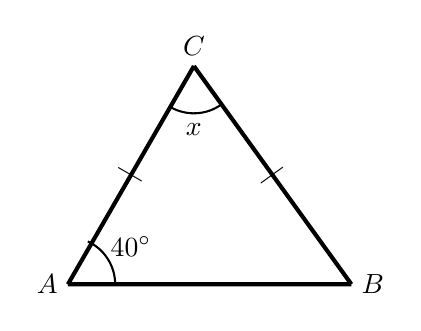
\begin{tikzpicture}[scale=0.8]
                \coordinate[label=left:$A$]  (A) at (0,0);
                \coordinate[label=right:$B$] (B) at (4.5,0);
                \coordinate[label=above:$C$] (C) at (2,3.464);
                %
                \draw(0,0) -- (0:0.75cm) arc (0:65:.75cm);
                \draw (1cm,0.6cm) node {$40^\circ$};
                %
                \begin{scope}[shift={(60:4)}]
                    \draw (0,0) -- (-120:.75cm) arc (-120:-55:.75cm);
                    \draw (-90:1cm) node {$x$};
                \end{scope}
                % triangle
                \draw [line width=1.5pt] (A) --  (B)
                                         (A) -- node[sloped] {$|$} (C)
                                         (B) -- node[sloped] {$|$} (C);
              \end{tikzpicture}
        \end{figure}
    \end{example}
\end{frame}
%%%%%%%%%%%%%%%%%%%%%%%%%%%%%%%%%%%%%%%%%%%%%%%%
%        SLIDE 
%%%%%%%%%%%%%%%%%%%%%%%%%%%%%%%%%%%%%%%%%%%%%%%%
\begin{frame}[t]{Example (Missing Angle)}
    \begin{example}
        Find $\angle x$.
            \begin{figure}[H]
                \centering
                

\tikzset{every picture/.style={line width=0.75pt}} %set default line width to 0.75pt        

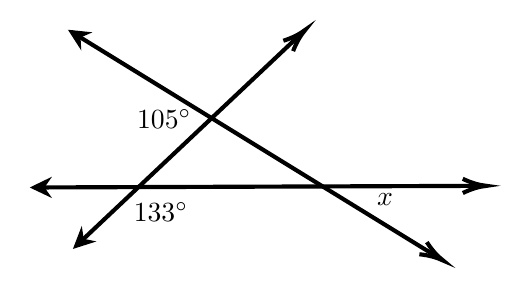
\begin{tikzpicture}[x=0.75pt,y=0.75pt,yscale=-1,xscale=1, scale=0.8]
%uncomment if require: \path (0,216); %set diagram left start at 0, and has height of 216

%Straight Lines [id:da6512016600166057] 
\draw [line width=1.5]    (181,119.99) -- (450,119.01) ;
\draw [shift={(453,119)}, rotate = 539.79] [color={rgb, 255:red, 0; green, 0; blue, 0 }  ][line width=1.5]    (14.21,-4.28) .. controls (9.04,-1.82) and (4.3,-0.39) .. (0,0) .. controls (4.3,0.39) and (9.04,1.82) .. (14.21,4.28)   ;
\draw [shift={(178,120)}, rotate = 359.79] [fill={rgb, 255:red, 0; green, 0; blue, 0 }  ][line width=1.5]  [draw opacity=0] (13.4,-6.43) -- (0,0) -- (13.4,6.44) -- (8.9,0) -- cycle    ;
%Straight Lines [id:da03571309045667914] 
\draw [line width=1.5]    (203.56,26.57) -- (424.44,162.43) ;
\draw [shift={(427,164)}, rotate = 211.59] [color={rgb, 255:red, 0; green, 0; blue, 0 }  ][line width=1.5]    (14.21,-4.28) .. controls (9.04,-1.82) and (4.3,-0.39) .. (0,0) .. controls (4.3,0.39) and (9.04,1.82) .. (14.21,4.28)   ;
\draw [shift={(201,25)}, rotate = 31.59] [fill={rgb, 255:red, 0; green, 0; blue, 0 }  ][line width=1.5]  [draw opacity=0] (13.4,-6.43) -- (0,0) -- (13.4,6.44) -- (8.9,0) -- cycle    ;
%Straight Lines [id:da32587616024700905] 
\draw [line width=1.5]    (206.18,154.94) -- (341.82,27.06) ;
\draw [shift={(344,25)}, rotate = 496.68] [color={rgb, 255:red, 0; green, 0; blue, 0 }  ][line width=1.5]    (14.21,-4.28) .. controls (9.04,-1.82) and (4.3,-0.39) .. (0,0) .. controls (4.3,0.39) and (9.04,1.82) .. (14.21,4.28)   ;
\draw [shift={(204,157)}, rotate = 316.68] [fill={rgb, 255:red, 0; green, 0; blue, 0 }  ][line width=1.5]  [draw opacity=0] (13.4,-6.43) -- (0,0) -- (13.4,6.44) -- (8.9,0) -- cycle    ;

% Text Node
\draw (392,127) node   {$x$};
% Text Node
\draw (257,135) node   {$133^{\circ }$};
% Text Node
\draw (259,79) node   {$105^{\circ }$};


\end{tikzpicture}
            \end{figure}
    \end{example}
\end{frame}

%%%%%%%%%%%%%%%%%%%%%%%%%%%%%%%%%%%%%%%%%%%%%%%%
%        SLIDE 
%%%%%%%%%%%%%%%%%%%%%%%%%%%%%%%%%%%%%%%%%%%%%%%%
\section{Quadrilaterals}
\begin{frame}{Quadrilaterals}
    \begin{itemize}
        \item We will discuss 5 common quadrilateral with some of their basic properties.
        \item Sum of interior angles in a quadrilateral is $360^\circ$.
    \end{itemize}
    %
    \begin{figure}[H]
        \centering
        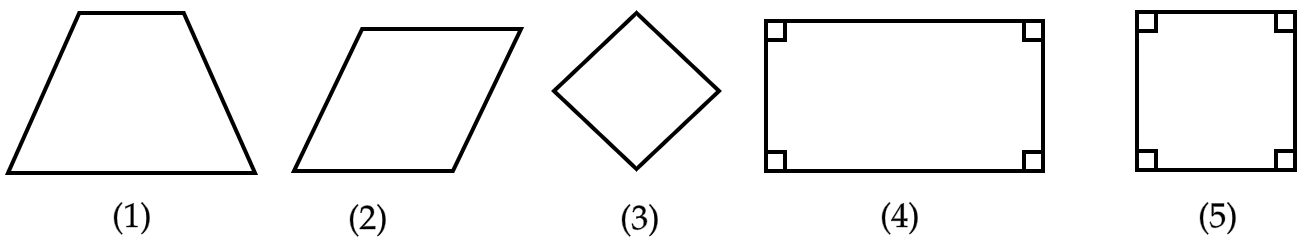
\includegraphics[scale=0.32]{pics/types_quadri.png}
    \end{figure}
\end{frame}
%%%%%%%%%%%%%%%%%%%%%%%%%%%%%%%%%%%%%%%%%%%%%%%%
%        SLIDE 
%%%%%%%%%%%%%%%%%%%%%%%%%%%%%%%%%%%%%%%%%%%%%%%%
\subsection{Trapezoid}
\begin{frame}{Trapezoid}
    \begin{itemize}
        \item Only two sides are parallel. 
        \item Those sides are called \textit{bases}.
    \end{itemize}
    %
    \begin{figure}[H]
        \centering
        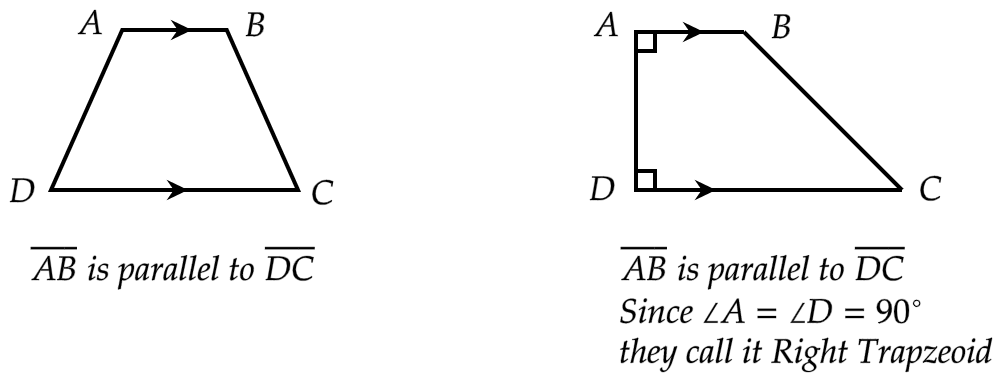
\includegraphics[scale=0.3]{pics/trapezoid.png}
    \end{figure}
\end{frame}
%%%%%%%%%%%%%%%%%%%%%%%%%%%%%%%%%%%%%%%%%%%%%%%%
%        SLIDE 
%%%%%%%%%%%%%%%%%%%%%%%%%%%%%%%%%%%%%%%%%%%%%%%%
\subsection{Parallelogram}
\begin{frame}{Parallelogram}
    \begin{itemize}
        \item Opposite sides are parallel.
        \item Opposite sides are equal.
    \end{itemize}
    %
    \begin{figure}[H]
        \centering
        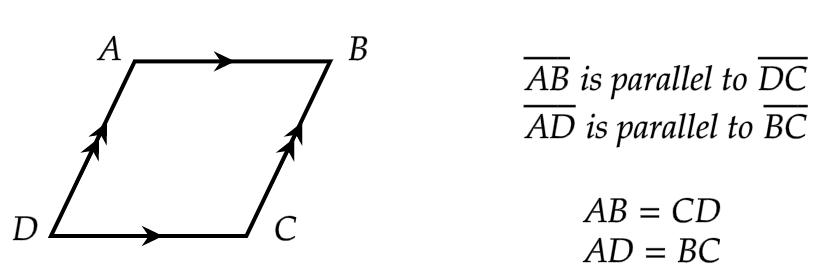
\includegraphics[scale=0.3]{pics/parallelogram.png}
    \end{figure}    
\end{frame}
%%%%%%%%%%%%%%%%%%%%%%%%%%%%%%%%%%%%%%%%%%%%%%%%
%        SLIDE 
%%%%%%%%%%%%%%%%%%%%%%%%%%%%%%%%%%%%%%%%%%%%%%%%
\subsection{Rhombus}
\begin{frame}{Rhombus (Diamond)}
    \begin{itemize}
        \item Opposite sides are parallel.
        \item All sides are equal.
    \end{itemize}
    %
    \begin{figure}[H]
        \centering
        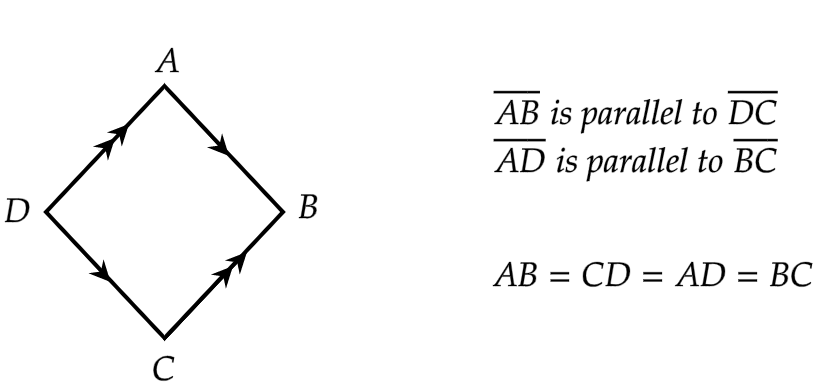
\includegraphics[scale=0.3]{pics/rhombus.png}
    \end{figure} 
\end{frame}
%%%%%%%%%%%%%%%%%%%%%%%%%%%%%%%%%%%%%%%%%%%%%%%%
%        SLIDE 
%%%%%%%%%%%%%%%%%%%%%%%%%%%%%%%%%%%%%%%%%%%%%%%%
\subsection{Rectangle}
\begin{frame}{Rectangle}
    \begin{itemize}
        \item Opposite sides are parallel.
        \item Opposite sides are equal.
        \item All angles are right angles (they are all $90^\circ$).
    \end{itemize}
    %
    \begin{figure}[H]
        \centering
        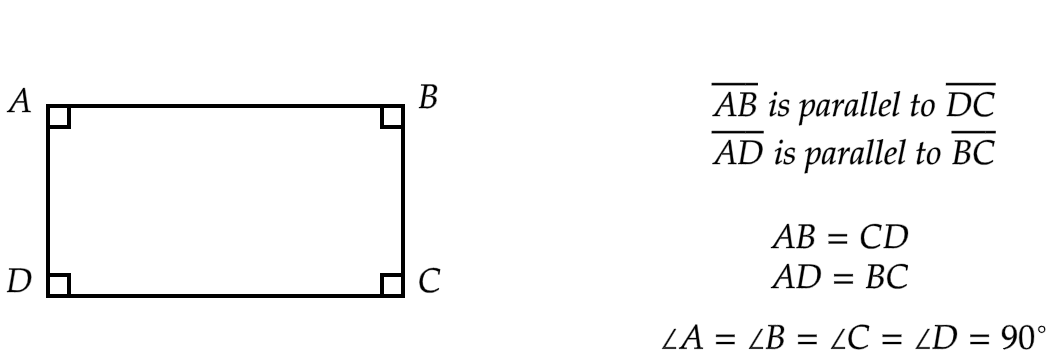
\includegraphics[scale=0.3]{pics/rectangle.png}
    \end{figure}   
\end{frame}
%%%%%%%%%%%%%%%%%%%%%%%%%%%%%%%%%%%%%%%%%%%%%%%%
%        SLIDE 
%%%%%%%%%%%%%%%%%%%%%%%%%%%%%%%%%%%%%%%%%%%%%%%%
\subsection{Square}
\begin{frame}{Square}
    \begin{itemize}
        \item Opposite sides are parallel.
        \item All sides are equal.
        \item All angles are right angles (they are all $90^\circ$).
    \end{itemize}
    %
    \begin{figure}[H]
        \centering
        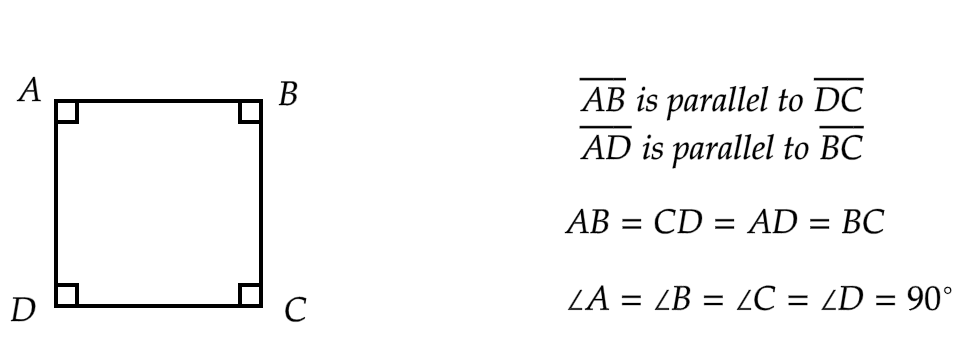
\includegraphics[scale=0.3]{pics/square.png}
    \end{figure}   
\end{frame}
%%%%%%%%%%%%%%%%%%%%%%%%%%%%%%%%%%%%%%%%%%%%%%%%
%        SLIDE 
%%%%%%%%%%%%%%%%%%%%%%%%%%%%%%%%%%%%%%%%%%%%%%%%
\begin{frame}[t]{Example (Find angles)}
    \begin{example}
        \begin{columns}[t]
        %
        \column{0.45\textwidth}
        Trapezoid $ABCD$ is shown below. 
        \begin{enumerate}[(a)]
            \item Determine $\angle x$.
            \item Determine $\angle y$.
        \end{enumerate}
        %
        \column{0.45\textwidth}
        \begin{figure}[H]
            \centering
            

\tikzset{every picture/.style={line width=0.75pt}} %set default line width to 0.75pt        

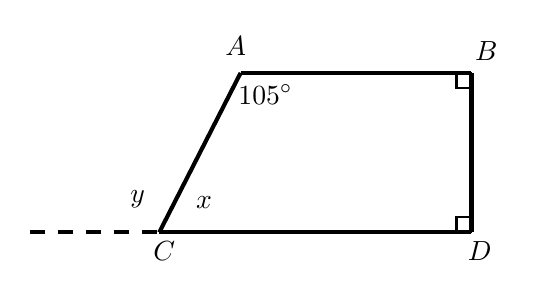
\begin{tikzpicture}[x=0.75pt,y=0.75pt,yscale=-1,xscale=1, scale=0.8]
%uncomment if require: \path (0,218); %set diagram left start at 0, and has height of 218

%Shape: Rectangle [id:dp392879367849994] 
\draw   (418,146) -- (427,146) -- (427,155) -- (418,155) -- cycle ;
%Shape: Rectangle [id:dp28556743489112235] 
\draw   (418,59) -- (427,59) -- (427,68) -- (418,68) -- cycle ;
%Straight Lines [id:da15725270794626356] 
\draw [line width=1.5]    (427,155) -- (239,155) ;


%Straight Lines [id:da6108314492525089] 
\draw [line width=1.5]    (427,155) -- (427,59) ;


%Straight Lines [id:da21099235794946036] 
\draw [line width=1.5]    (288,59) -- (427,59) ;


%Straight Lines [id:da9882398763880909] 
\draw [line width=1.5]    (239,155) -- (288,59) ;


%Straight Lines [id:da2719389491415545] 
\draw [line width=1.5]  [dash pattern={on 5.63pt off 4.5pt}]  (161,155) -- (239,155) ;



% Text Node
\draw (285,43) node   {$A$};
% Text Node
\draw (436,46) node   {$B$};
% Text Node
\draw (242,166) node   {$C$};
% Text Node
\draw (432,166) node   {$D$};
% Text Node
\draw (303,72) node   {$105^{\circ }$};
% Text Node
\draw (266,137) node   {$x$};
% Text Node
\draw (226,135) node   {$y$};


\end{tikzpicture}
        \end{figure}
        %
        \end{columns}
    \end{example}
\end{frame}